\title{Warm-Up for April 13th, 2022}
\author{Dr. Jordan Hanson - Whittier College Dept. of Physics and Astronomy}
\date{\today}
\documentclass[12pt]{article}
\usepackage[a4paper, total={18cm, 27cm}]{geometry}
\usepackage{graphicx}
\usepackage{amsmath}
\usepackage{subcaption}
\usepackage{bm}
\def\rcurs{{\mbox{$\resizebox{.16in}{.08in}{
\includegraphics{ScriptR}}$}}}
\def\brcurs{{\mbox{$\resizebox{.16in}{.08in}{
\includegraphics{BoldR}}$}}}
\def\hrcurs{{\mbox{$\hat \brcurs$}}}
 
\begin{document}
\maketitle
\small
\section{Memory Bank}
\begin{enumerate}
\item Amp\`{e}re's Law with $\mathbf{B}$-fields, $\mathbf{A}$-fields.
\begin{align}
\nabla \times \mathbf{B} &= \mu_0 \mathbf{J} \label{eq:1} \\
\nabla^2 \mathbf{A} &= -\mu_0 \mathbf{J} \label{eq:2} 
\end{align}
\end{enumerate}

\begin{figure}[ht]
\centering
\begin{subfigure}{0.12\textwidth}
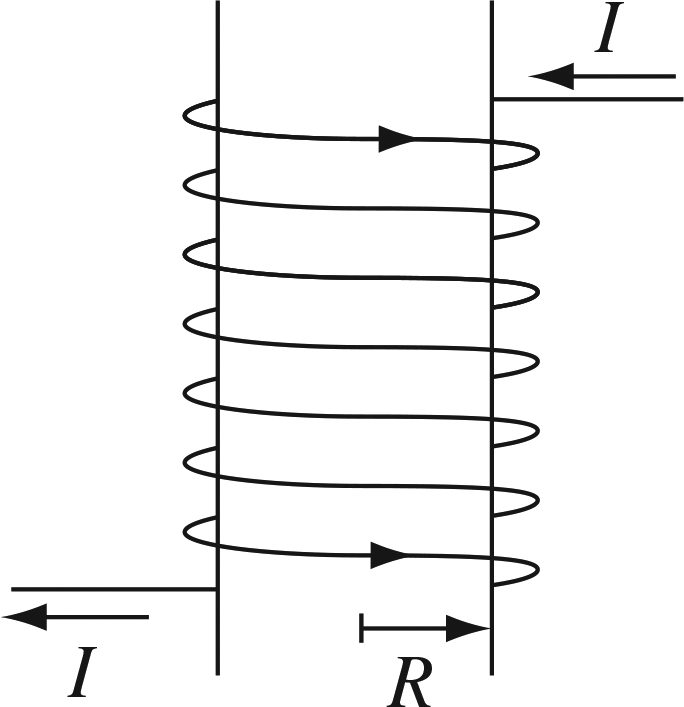
\includegraphics[width=\textwidth]{figures/5_34.jpg}
\caption{ }
\end{subfigure}
\hfill
\begin{subfigure}{0.07\textwidth}
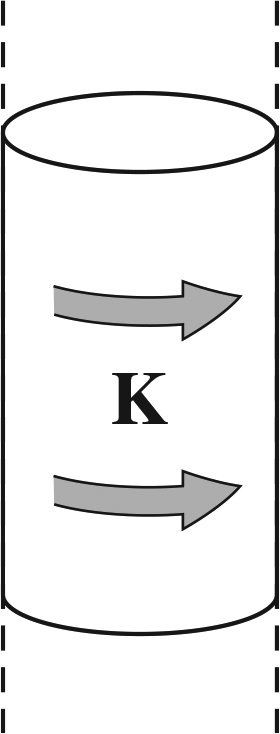
\includegraphics[width=\textwidth]{figures/5_35.jpg}
\caption{ }
\end{subfigure}
\hfill
\begin{subfigure}{0.2\textwidth}
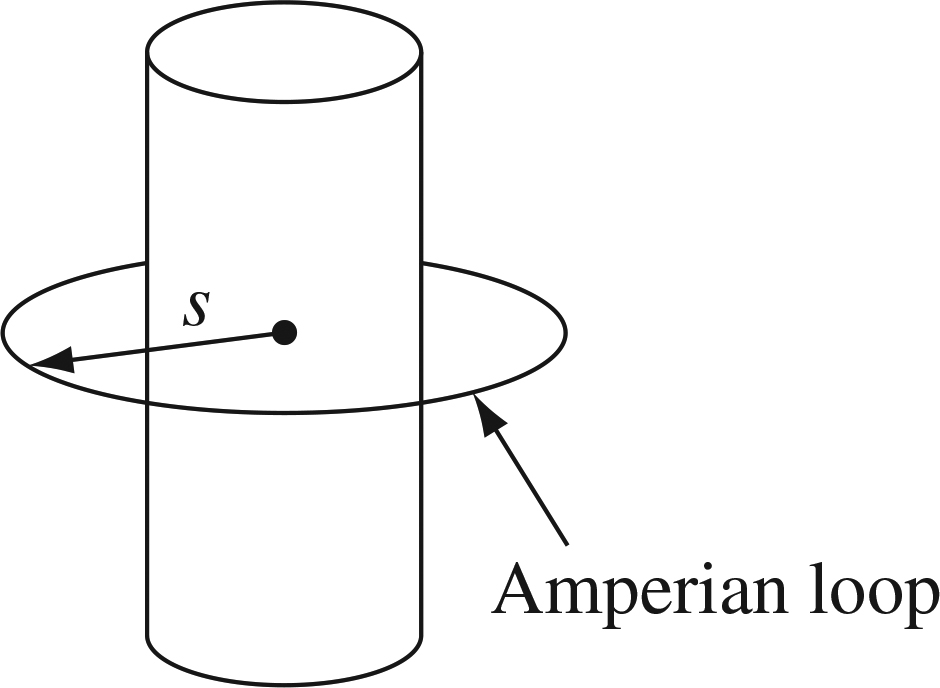
\includegraphics[width=\textwidth]{figures/5_36.jpg}
\caption{ }
\end{subfigure}
\hfill
\begin{subfigure}{0.15\textwidth}
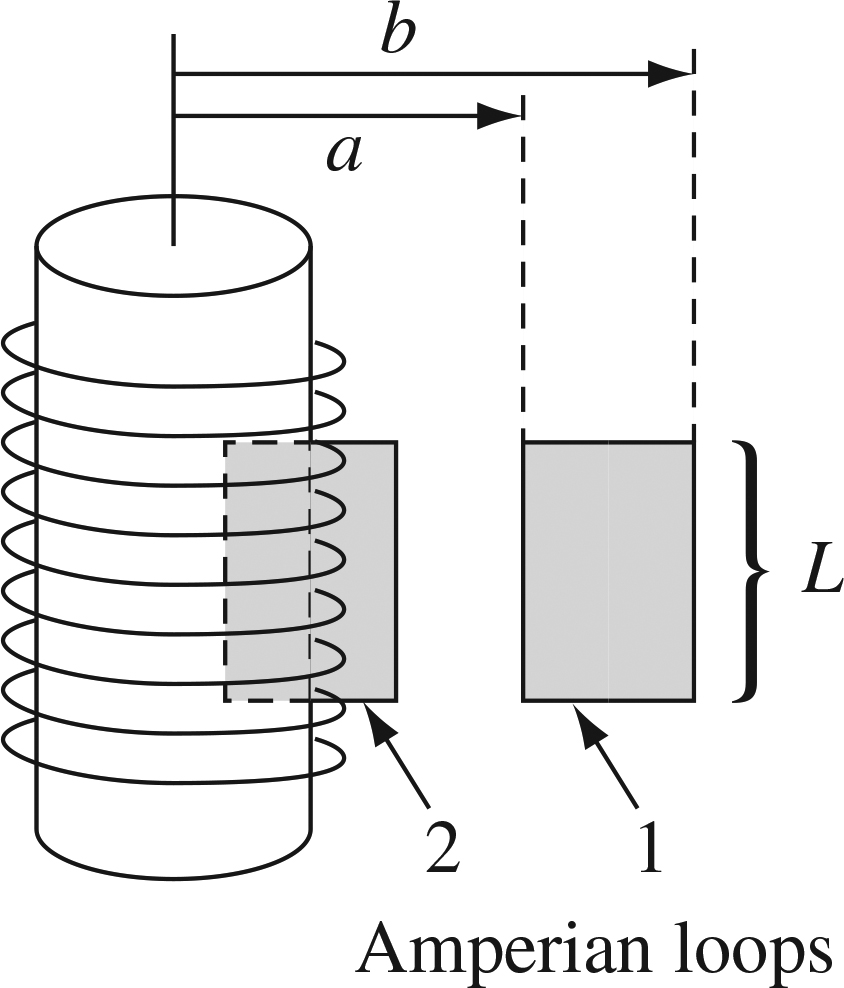
\includegraphics[width=\textwidth]{figures/5_37.jpg}
\caption{ }
\end{subfigure}
\caption{\label{fig:1} (a) A current wound around a solid cylinder is called a solenoid.  (b) This leads to a surface current $\mathbf{K}$. (c) An Amperian loop aids in finding the $\mathbf{B}$-field. (d) Loops inside and outside determine where $\mathbf{B} \neq 0$.}
\end{figure}

\section{B-fields and A-fields with Solenoids}

\begin{enumerate}
\item Consider Fig. \ref{fig:1}.  A cylindrical current is called a \textit{solenoid}.  (a) Using geometric arguments, prove that the field inside the solenoid is strictly in the $\hat{\mathbf{z}}$ direction (parallel to the cylinder). Use Fig. \ref{fig:1} (c) to show that $B_\phi = 0$. (b) The surface current density is $\mathbf{K} = n I\hat{\boldsymbol\phi}$, where $n = N/L$, the turns per unit length.  Use the integral form of Amp\`{e}re's Law to show that $\mathbf{B} = \mu_0 n I\hat{\mathbf{z}}$ inside the cylinder. \\ \vspace{2cm}
\item The definition of the \textit{vector potential} is $\mathbf{B} = \nabla \times \mathbf{A}$, because $\nabla \cdot \mathbf{B} = 0$. (a) Perform a surface integral on both sides of the definition of $\mathbf{A}$ and use the curl-theorem to show that $\oint \mathbf{A} \cdot d\mathbf{l} = \int \mathbf{B} \cdot d\mathbf{a} = \Phi_B$. Obtain $\mathbf{A}$ for the solenoid inside and out, using $\mathbf{B}$. \footnote{You may assume $\mathbf{A}$ is parallel to the current.  See Eq. 5.65 in the text.}
\end{enumerate}
\end{document}